\section{Tests}
\label{section:tests}

\subsection{Type of tests}

\subsubsection{JUnit}

\begin{figure}[h]
	\centering
	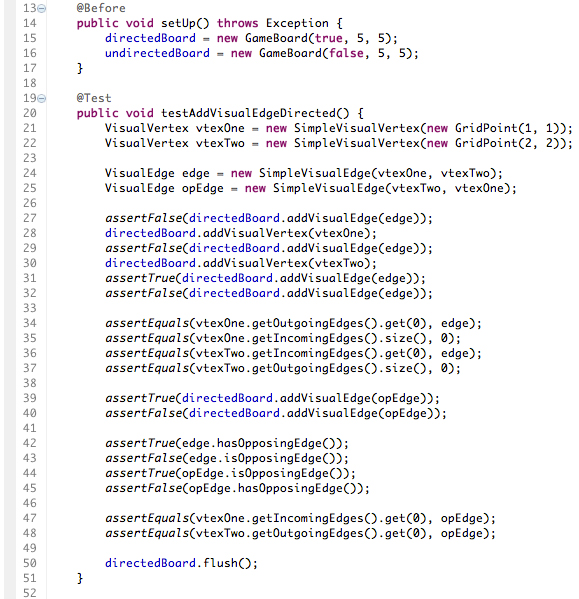
\includegraphics[width=.95\textwidth]{junit_screenshot.jpg}
	\caption{JUnit test for the GameBoard.}
	\label{img:screenJUnit}
\end{figure}
\emph{JUnit} is the most commonly used framework to write repeatable unit tests for Java applications.\par
Every object can be tested separately using defined input values and expected output values. Methods and object correlations not working as intended will attract attention reliably.\par

\subsubsection{Algorithms}

\todo{Algorithms section}

\subsubsection{Sikuli}

\begin{figure}[!h]
	\centering
	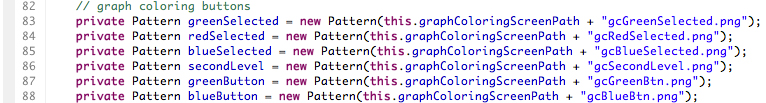
\includegraphics[width=.95\textwidth]{sikuli_screenshot_1.jpg}
	\caption{GUI elements defined for tests with Sikuli.}
	\label{img:screenSikuli1}
\end{figure}
\begin{figure}[!h]
	\centering
	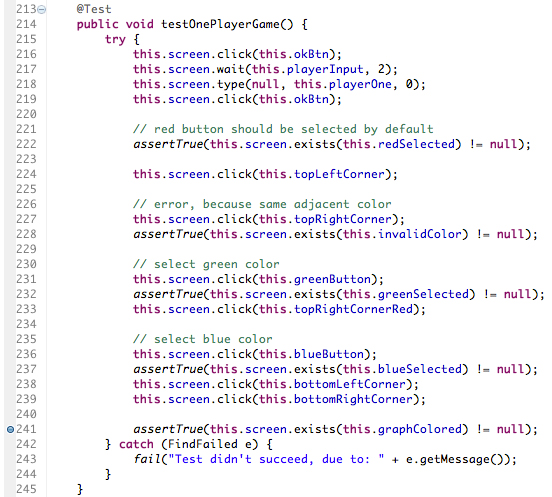
\includegraphics[width=.95\textwidth]{sikuli_screenshot_2.jpg}
	\caption{Sikuli test for the Graph-Coloring single-player game.}
	\label{img:screenSikuli2}
\end{figure}
For extensive tests of our graphical user interfaces (GUIs), we drew on open-source \emph{Project SIKULI}. Sikuli is a visual technology to automate and test those interfaces using screenshots.\par
Sikuli itself is written in Java and is being used by importing the Sikuli library.\par
With Sikuli every possible item can be clicked on, no matter if its a real button, text field etc. The program simply looks for the provided screenshot in the GUI and simulates a mouse click or key stroke on the item that it found. In Java code the test developer then defines click paths, key input, and assertions. An example for this is outlined in Fig. \ref{img:screenSikuli2}.\par
Those assertions again are cropped images from screenshots. If they appear somewhere after the click, the test passes, otherwise it fails.\par
Once all clickable items are saved as screenshot parts (see Fig. \ref{img:screenSikuli1}), every possible scenario can be executed semi-automatically. These tests can also be designed as regression test.\par
With Sikuli one can only test visual existence or non-existence of a given object. For example if the execution of the help page calls 10 different methods, Sikuli is not able to test if the methods are correct, but can only verify if the end result is as expected.\par

\subsubsection{Manual tests}

As defined in the \emph{Pflichtenheft}, we conducted 18 test cases and four test scenarios. As those have been defined before design and implementation, they give some indication of whether the framework and the games in general have been deployed as planned.\par

\subsection{Implementation details}
We implemented unit tests during the implementation phase, achieving a code coverage between 76\% and 98\%, depending on the packages.\par
A lot more unit test have been added since and by the end of the validation phase, we beat the number of 98\% \todo{Verify number} of code coverage with unit tests, GUI tests and manual tests all together.\par
However, a lot of possible errors could be embedded in the GUIs. And as Java does not provide easy and free frameworks for GUI testing, we used the above described Sikuli to act out almost all possible click and key combinations in both \gameexplorer and \emph{GameWindow}.\par
The - mainly positive - results of all tests are outlined in the next sections.\par
